\documentclass[11pt]{article}
\usepackage[margin=1in]{geometry}
\usepackage{booktabs}
\usepackage{graphicx}
\usepackage{amsmath}
\usepackage{caption}
\captionsetup{font=small,skip=6pt}

\title{MVP: a pseudo-outcome tax on a bandit of deployed scores\\
\large Gradual relocation only. Saved to continue later.}
\author{}
\date{}

\begin{document}
\maketitle

\section{The piece worth keeping}

Four linear scorecards are arms. The reward is negative batch mean squared error.
A standard index (UCB, discounted UCB, or a Thompson draw) is reduced by
\(\eta\sigma w_k\), where \(w_k\) is the FSDS pseudo-outcome risk share of arm \(k\)
and \(\sigma\) is the scale of the four arm rewards on a reference window.
\(\eta\in\{0.5,1,2\}\). Nothing in this note uses \(\lambda=20\) or \(40\).

The share is the held-out residual variance of a doubly robust pseudo-outcome,
divided by the sum of those residuals. The two windows are the first six batches
and the latest six. It is refreshed every eight rounds from round 16, from every
scorecard's prediction on the logged batch. Serving a scorecard is not required
to score it.

The environment is a ramp. The mixing weight is \(0\) through round \(20\) and
then linear to \(1\). The next batch is not announced. There is no change-point
indicator, and a jump is not part of this MVP.

On a gradual relocation the tax earns its keep. The median post-shift excess,
across six pools, is \(17.6\) for UCB at \(\eta=2\), against \(34.6\) for UCB,
\(24.6\) for discounted UCB, and \(125\) for \(\varepsilon\)-greedy at \(10\%\).
The same gap clears the larger seed standard deviation on all six pools against
UCB, on five pools against discounted UCB, and on all six against
\(\varepsilon=0.10\). The early window, before the ramp, is unchanged: the tax
does not spend exploratory batches while the relevant arm already wins the reward.

\section{What the share is screening}

The share does not follow the scorecard whose predictions moved the most.
It follows the scorecard that has stopped explaining \(y\).

\begin{figure}[ht]
\centering
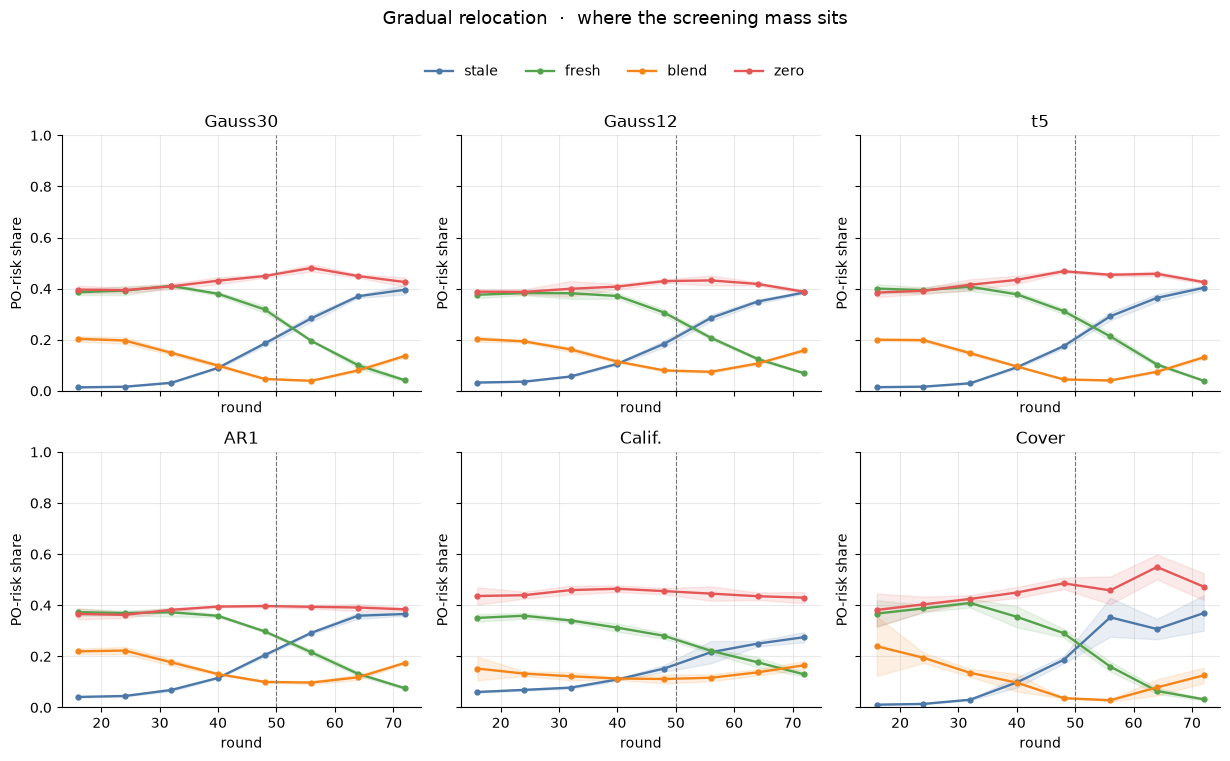
\includegraphics[width=\textwidth]{figures/shares_gradual_relocate.png}
\caption{Shares on a gradual relocation, mean over four seeds.
Before the ramp the fresh block and the zero score hold the mass.
After the mixing weight passes \(1/2\) (dashed line) the fresh share falls
and the stale share rises. The crossing is on all six pools.}
\end{figure}

Before the move, \(y\) lives on the stale block, so that score absorbs the
pseudo-outcome and its residual share is small. The fresh block and the zero
score do not explain \(y\), so they carry the tax. After the move the fresh
residual collapses and the stale residual inflates. An arm that the ramp has
moved onto sheds the tax. An arm that moved against the world, or never carried
the signal, keeps it.

\begin{figure}[ht]
\centering
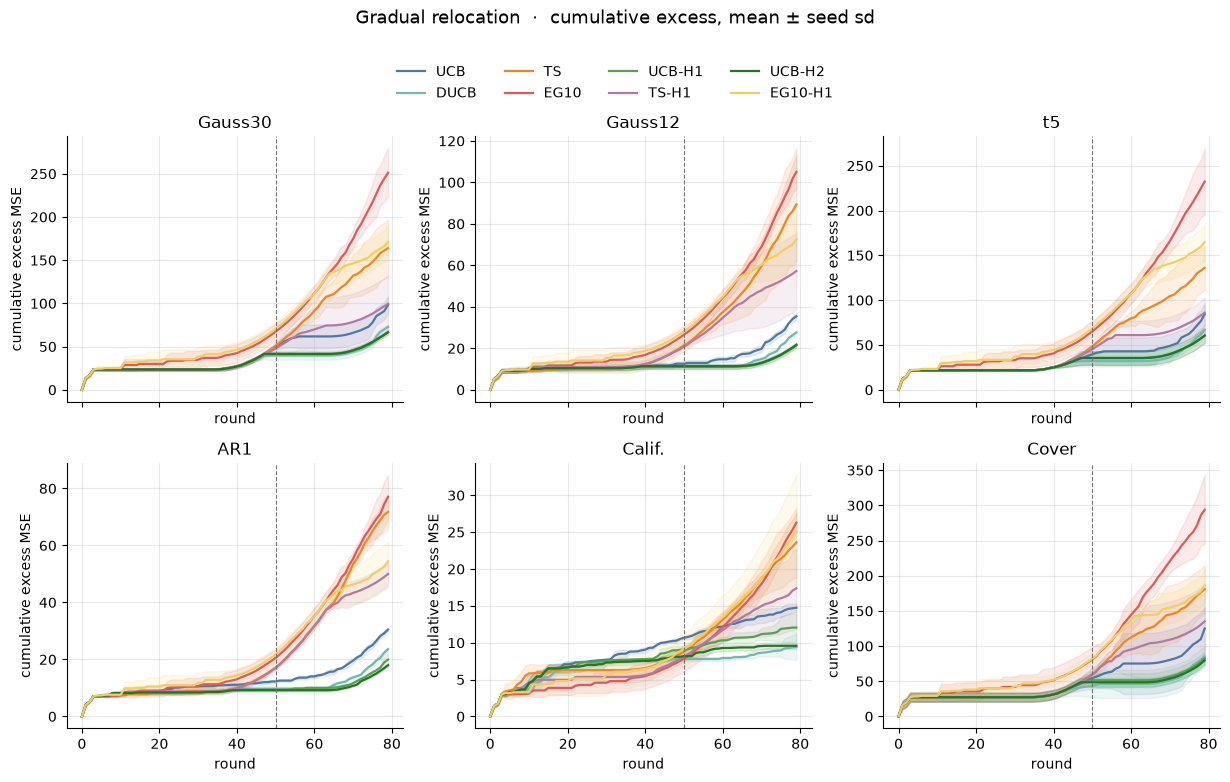
\includegraphics[width=\textwidth]{figures/cum_gradual_relocate.png}
\caption{Cumulative excess on a gradual relocation.
UCB at \(\eta=1\) or \(2\) flattens after the dashed line.
\(\varepsilon\)-greedy at \(10\%\) keeps accumulating.}
\end{figure}

\section{Pool by pool}

Post-shift excess MSE. Mean over seeds \(20261018\)--\(20261021\).
Parentheses are the seed standard deviation.
A cut is \((\mathrm{UCB}-\mathrm{taxed})/\mathrm{UCB}\).

\begin{center}
\begin{tabular}{lcccc}
\toprule
Pool & UCB & dUCB & UCB \(\eta=2\) & cut \\
\midrule
Gaussian \(d=30\) & 50.61 (8.51) & 32.71 (6.18) & 25.12 (1.51) & 50\% \\
Gaussian \(d=12\) & 22.87 (0.43) & 16.43 (1.31) & 10.31 (0.13) & 55\% \\
Student-\(t_5\) & 46.29 (4.72) & 34.85 (3.66) & 24.98 (1.09) & 46\% \\
AR(1), \(\rho=0.6\) & 18.22 (1.10) & 13.86 (0.66) & 8.80 (0.52) & 52\% \\
California housing & 4.23 (0.63) & 1.65 (1.50) & 1.49 (0.58) & 65\% \\
Covertype & 73.10 (20.68) & 42.22 (0.64) & 31.17 (1.16) & 57\% \\
\bottomrule
\end{tabular}
\end{center}

California against discounting alone sits inside the seed noise
(\(1.65\) with sd \(1.50\), tax \(1.49\)). That pool has eight columns, so the
blocks are short. Everywhere else the gap against discounting also clears the
seed noise. The taxed seed sd is smaller on every pool. Covertype falls from
\(20.7\) to \(1.2\).

The hit rate only moves from about \(0.38\)--\(0.44\) to about \(0.47\)--\(0.51\)
on the large synthetic pools. Excess falls by half because the rule stops
serving the stale card and the zero card. The blend, close to the fresh block
during the ramp, takes many of the remaining rounds. \(\varepsilon=0.10\) hits
the best card on about \(0.03\) of post-shift rounds.

\section{Policies, the deployable monitor}

The same share on four linear policies, horizon \(4\), \(200\) episodes a round,
same ramp. Phase-1 median excess return on a single block move:
UCB at \(\eta=2\) is \(7.1\), discounted UCB is \(16.0\), plain UCB is \(32.0\),
\(\varepsilon=0.10\) is \(54.4\).

The oracle share sees every policy's return. The version that can be deployed
fits the reward on the served transitions, imagines the other policies, and
then computes the share. On the second move of a two-block ramp its phase-2
median is \(14.6\) at \(\eta=1\), next to the oracle tax at \(\eta=2\) (\(11.0\))
and below discounted UCB (\(16.4\)) and plain UCB (\(42.6\)).

Assigning residual \(1\) to a policy that was not served does not survive that
second move. Its phase-2 median is \(96\), worse than plain UCB. Missing is not
the same thing as unexplained.

\section{Where this MVP stops}

A gradual sign flip is the shut-off. The two signed scores stay nearly tied and
the zero score holds about \(0.38\) to \(0.58\) of the share, so the tax pushes
away from the hedge. Discounted UCB, tax off, has median post excess \(99.2\).
UCB at \(\eta=1\) is \(185\). The shut-off is visible in the weights: one null
score holds the mass and the live scores are tied. Set \(\eta=0\).

A dying block and a nonlinear add-on have better medians with discounted UCB at
\(\eta=2\) (\(27.1\) and \(2.80\)) than with discounting alone, but the per-pool
gap over discounting is often inside the seed noise. They are not the claim.
Noise growth is a small positive result for Thompson sampling with a light tax
(median \(0.90\) at \(\lambda=5\), \(1.16\) at \(\eta=2\), against \(3.97\) for
UCB). Discounting hurts there, because the best card never changed.

Jumps are a different problem. On a sudden relocation the best median is plain
discounted UCB. They are logged in the long note and are not this MVP.

\section{Continue from here}

The long write-up, every table, and the figure set are
\texttt{fsds\_porisk\_note.pdf} in this directory.
The runners are \texttt{Python/run\_fsds\_porisk\_poc.py},
\texttt{Python/fsds\_porisk\_lib.py}, and \texttt{Python/fsds\_policy\_lib.py}.
Batches are \(200\) rows, \(80\) rounds, reference window \(6\), refresh every
\(8\) from round \(16\). Pools are the two Gaussians, Student-\(t_5\), AR(1),
California housing, and a \(30{,}000\)-row Covertype draw.

Three things are concrete enough to pick up.
First, read the shut-off off the share itself, before looking at regret, and
turn the tax off when a null score holds the mass.
Second, keep the reward fit that imagines unserved policies. Do not impute a
residual for a policy the log never saw.
Third, keep \(\eta\sigma\) rather than a raw \(\lambda\). One \(\eta\) in
\(\{1,2\}\) travels across these pools. One raw \(\lambda\) does not, and
\(\eta>2\) is the direction that breaks the sign-flip hedge.

\end{document}
